% =============================================================
% Seminar Proposal Tesis
% CNN–Transformer Encoder–Decoder for LIBS Spectral Analysis
% of Volcanic Soil
% =============================================================

\documentclass{beamer}
\usepackage[en]{zafu}

% Charts & diagrams
\usepackage{pgfplots}
\usetikzlibrary{positioning, arrows.meta, shapes.geometric, calc, fit}
\pgfplotsset{compat=1.17}
\usepackage{booktabs}
\usepackage{array}

% Slightly smaller author & affiliation on title page
\setbeamerfont{author}{size=\small}
\setbeamerfont{institute}{size=\footnotesize}
\setbeamerfont{date}{size=\footnotesize}

% PDF metadata
\hypersetup{
  pdftitle={CNN-Transformer Encoder-Decoder for LIBS Spectral Analysis of Volcanic Soil},
  pdfauthor={Birrul Walidain},
  pdfsubject={LIBS; CNN-Transformer; Encoder-Decoder; Volcanic Soil},
  pdfkeywords={LIBS, CNN, Transformer, Encoder-Decoder, Volcanic Soil, Spectroscopy}
}
\pdfstringdefDisableCommands{%%
  \def\\{}%%
  \def\textsuperscript#1{#1}%%
}

% ----- Metadata -----
\title[CNN--Transformer LIBS]{%
  Spectral Reconstruction in\\ Laser-Induced Breakdown Spectroscopy\\
  Using a CNN--Transformer Encoder--Decoder:\\
  Application to Volcanic Soil}

\subtitle{Seminar Proposal Tesis}

\author[B.\,Walidain]{%
  Birrul Walidain\\[2pt]
  {\footnotesize NPM: 250820201100015}}

\institute{%
  \footnotesize
  Program Studi Magister Fisika\\
  Fakultas MIPA, Universitas Syiah Kuala\\[6pt]
  {\scriptsize
    Pembimbing I: Prof.\ Dr.\ Eng.\ Nasrullah, S.Si., M.T.\\
    Pembimbing II: Dr.\ Khairun Saddami, S.T.}}

\date{\today}

\titlegraphic{\includegraphics[width=0.16\textwidth]{src/logo-usk.png}}

% =============================================================
\begin{document}

% Slide 1: Title
\maketitle

% =============================================================
% Slide 2: Janji & Tujuan
% =============================================================
\begin{frame}{Promise \& Purpose}
  \textbf{In the next 15 minutes, you will understand:}
  \vspace{0.6em}

  \centering
  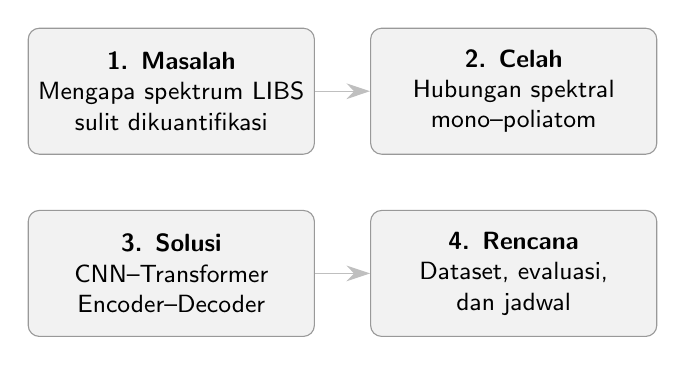
\begin{tikzpicture}[node distance=0.7cm and 0.7cm]
    \tikzset{
      box/.style={
        rectangle, rounded corners,
        draw=black!40, fill=gray!10,
        text width=3.4cm, align=center,
        minimum height=1.6cm, font=\small\sffamily
      }
    }

    % Row 1
    \node[box] (b1) {\textbf{1. Masalah}\\Mengapa spektrum LIBS\\sulit dikuantifikasi};
    \node[box, right=of b1] (b2) {\textbf{2. Celah}\\Hubungan spektral\\mono--poliatom};

    % Row 2
    \node[box, below=of b1] (b3) {\textbf{3. Solusi}\\CNN--Transformer\\Encoder--Decoder};
    \node[box, below=of b2] (b4) {\textbf{4. Rencana}\\Dataset, evaluasi,\\dan jadwal};

    \draw[-{Stealth[length=3mm,width=2mm]},gray!50] (b1) -- (b2);
    \draw[-{Stealth[length=3mm,width=2mm]},gray!50] (b3) -- (b4);
  \end{tikzpicture}

  \vspace{0.6em}
  \textbf{Tujuan:} Kerangka \textit{deep learning} yang secara eksplisit memodelkan komposisi spektral mono--poliatom untuk analisis kuantitatif LIBS pada tanah vulkanik.
\end{frame}

% =============================================================
% Slide 3: Peta Jalan & Batasan
% =============================================================
\section{Introduction}

\begin{frame}{Roadmap \& Fence}
  \textbf{Agenda}
  \begin{enumerate}\setlength{\itemsep}{1pt}
    \item \textbf{Masalah:} Kompleksitas spektral \& tantangan kuantifikasi.
    \item \textbf{Celah:} Hubungan spektral mono--poliatom belum dimodelkan.
    \item \textbf{Solusi:} Arsitektur CNN--Transformer Encoder--Decoder.
    \item \textbf{Rencana:} Dataset, metrik evaluasi, \& jadwal penelitian.
  \end{enumerate}
  \vspace{0.4em}
  \textbf{Scope (Fence)}
  \begin{itemize}\setlength{\itemsep}{1pt}
    \item Asumsi plasma LTE; jendela spektral 200--900\,nm.
    \item Data sintetis melalui Saha--Boltzmann + transisi NIST ASD.
    \item Validasi eksperimental pada tanah vulkanik (wilayah Aceh).
    \item Regresi kuantitatif (prediksi konsentrasi), bukan klasifikasi.
  \end{itemize}
\end{frame}

% =============================================================
% Slide 4: Masalah — Mengapa Kuantifikasi LIBS Sulit
% =============================================================
\begin{frame}{Problem: Why Quantification in LIBS is Hard}
  \begin{columns}[T,onlytextwidth]
    \begin{column}{0.45\textwidth}
      {\footnotesize
      \textbf{Kompleksitas \& Kalibrasi}
      \begin{itemize}\setlength{\itemsep}{0pt}
        \item Spektrum poliatom: tumpang tindih emisi kompleks.
        \item Dinamika plasma fluktuatif.
        \item \textit{Self-absorption} \& \textit{continuum noise}.
        \item CRM langka; regresi empiris gagal di sampel heterogen.
      \end{itemize}
      
      \vspace{0.3em}
      \textbf{Wawasan (\(\rightarrow\) Implikasi)}
      \begin{quote}
        \raggedright \setlength{\baselineskip}{0.9\baselineskip}
        Spektrum LIBS bukan sinyal sederhana, melainkan \textbf{komposisi spektrum monoatom}. Model konvensional mengabaikan \emph{struktur} ini.
      \end{quote}
      }
    \end{column}
    \begin{column}{0.53\textwidth}
      \centering
      \vspace{0pt}
      \includegraphics[width=\textwidth,height=0.85\textheight,keepaspectratio]{gallery/slide/libs_4panel.png}
    \end{column}
  \end{columns}
\end{frame}

% =============================================================
% Slide 5: Penelitian Sebelumnya (Tabel Ringkas) (Dihapus)
% =============================================================
\iffalse
\begin{frame}{Previous Research}
  \centering
  \scriptsize
  \renewcommand{\arraystretch}{1.3}
  \begin{tabular}{>{\raggedright\arraybackslash}p{2.0cm} >{\raggedright\arraybackslash}p{2.3cm} >{\raggedright\arraybackslash}p{3.2cm} >{\raggedright\arraybackslash}p{3.8cm}}
    \toprule
    \textbf{Peneliti} & \textbf{Metode} & \textbf{Kontribusi} & \textbf{Keterbatasan} \\
    \midrule
    Favre et~al. (2025) &
      Radiative transfer (LTE) &
      Simulasi spektrum berbasis fisika plasma &
      Komputasi mahal; hanya model \textit{forward} \\
    \addlinespace
    Favre et~al. (2025) &
      CNN untuk CF-LIBS &
      Prediksi komposisi unsur secara \textit{real-time} &
      Spektrum diperlakukan sebagai vektor tunggal \\
    \addlinespace
    Liu et~al. (2026) &
      Transformer--CNN &
      Analisis unsur jejak pada LIBS jarak jauh &
      Belum memisahkan spektrum mono/poliatom \\
    \addlinespace
    Walidain et~al. (2026) &
      Informer &
      Identifikasi multi-elemen kualitatif &
      Hanya klasifikasi; belum regresi \\
    \bottomrule
  \end{tabular}

  \vspace{0.6em}
  {\small \textbf{Keterbatasan umum:} Semua pendekatan memperlakukan spektrum sebagai \emph{sinyal tunggal} tanpa memodelkan komposisi mono--poliatom.}
\end{frame}
\fi


% =============================================================
% Slide 5a: Deep Dive Literature 1 (2x2 Flowchart)
% =============================================================
\begin{frame}{Previous Research}
  \framesubtitle{Favre et al. (2025) --- MERLIN \textit{(Physics Simulation)}}
  \centering  
  \tikzset{
    flowbox/.style={rectangle, draw=black!60, fill=gray!10, rounded corners=1mm,
      text width=4.8cm, align=center, font=\small\sffamily, minimum height=1.3cm, inner sep=2mm},
    gapbox/.style={flowbox, fill=red!8, draw=red!50},
    impbox/.style={rectangle, draw=orange!80!black, fill=orange!10, rounded corners=1mm,
      text width=10.4cm, align=center, font=\small\sffamily\bfseries, minimum height=0.8cm, inner sep=2mm},
    arrow/.style={-{Stealth[length=3mm,width=2mm]}, thick, draw=black!60}
  }

  \begin{tikzpicture}[node distance=0.2cm and 0.4cm]
    \node[flowbox] (p1) {\textbf{Problem}\\[0.5em] \footnotesize CF-LIBS butuh model plasma realistis untuk pemetaan \textit{spectral emission}.};
    \node[flowbox, right=of p1] (m1) {\textbf{Method}\\[0.5em] \footnotesize Simulasi \textit{radiative transfer} fisik MERLIN via basis data NIST (LTE).};
    
    \node[flowbox, below=of m1] (i1) {\textbf{Insight}\\[0.5em] \footnotesize Sukses visualisasi \textit{self-absorption} optik tebal \& \textit{line broadening}.};
    \node[gapbox, left=of i1] (g1) {\textbf{Gap}\\[0.5em] \footnotesize Eksklusif menyelesaikan \textbf{forward problem}, belum mampu \textbf{inverse}.};
    
    \node[impbox, below=0.3cm of g1.south west, anchor=north west] (imp1) {Implikasi Tesis: Butuh \textit{ML surrogate} untuk iterasi \textit{inverse} mereduksi beban analitik.};
    
    \draw[arrow] (p1) -- (m1);
    \draw[arrow] (m1) -- (i1);
    \draw[arrow] (i1) -- (g1);
    \draw[arrow, draw=orange!80, thick] (g1.south) -- (g1.south |- imp1.north);
  \end{tikzpicture}
\end{frame}

% =============================================================
% Slide 5b: Deep Dive Literature 2 (2x2 Flowchart)
% =============================================================
\begin{frame}{Previous Research}
  \framesubtitle{Walidain et al. (2026) --- Informer \textit{(Qualitative DL)}}
  \centering  
  \tikzset{
    flowbox/.style={rectangle, draw=black!60, fill=gray!10, rounded corners=1mm,
      text width=4.8cm, align=center, font=\small\sffamily, minimum height=1.3cm, inner sep=2mm},
    gapbox/.style={flowbox, fill=red!8, draw=red!50},
    impbox/.style={rectangle, draw=orange!80!black, fill=orange!10, rounded corners=1mm,
      text width=10.4cm, align=center, font=\small\sffamily\bfseries, minimum height=0.8cm, inner sep=2mm},
    arrow/.style={-{Stealth[length=3mm,width=2mm]}, thick, draw=black!60}
  }

  \begin{tikzpicture}[node distance=0.2cm and 0.4cm]
    \node[flowbox] (p1) {\textbf{Problem}\\[0.5em] \footnotesize Rentang spektrum emisi LIBS berdimensi sangat besar.};
    \node[flowbox, right=of p1] (m1) {\textbf{Method}\\[0.5em] \footnotesize \textit{Informer Transformer} dengan mekanisme \textit{ProbSparse Self-Attention}.};
    
    \node[flowbox, below=of m1] (i1) {\textbf{Insight}\\[0.5em] \footnotesize Atensi spasial efektif rotasi tangkap \textit{wavelength dependency} korelasi spektral.};
    \node[gapbox, left=of i1] (g1) {\textbf{Gap}\\[0.5em] \footnotesize Hanya model \textbf{Klasifikasi Kualitatif}, gagal regresi konsentrasi kuantitatif.};
    
    \node[impbox, below=0.3cm of g1.south west, anchor=north west] (imp1) {Implikasi Tesis: Modifikasi arsitektur murni untuk mengeksekusi \textit{Quantitative Regression}.};
    
    \draw[arrow] (p1) -- (m1);
    \draw[arrow] (m1) -- (i1);
    \draw[arrow] (i1) -- (g1);
    \draw[arrow, draw=orange!80, thick] (g1.south) -- (g1.south |- imp1.north);
  \end{tikzpicture}
\end{frame}

% =============================================================
% Slide 5c: Deep Dive Literature 3 (2x2 Flowchart)
% =============================================================
\begin{frame}{Previous Research}
  \framesubtitle{Liu et al. (2026) --- TransCNN \textit{(Quantitative Hybrid DL)}}
  \centering  
  \tikzset{
    flowbox/.style={rectangle, draw=black!60, fill=gray!10, rounded corners=1mm,
      text width=4.8cm, align=center, font=\small\sffamily, minimum height=1.3cm, inner sep=2mm},
    gapbox/.style={flowbox, fill=red!8, draw=red!50},
    impbox/.style={rectangle, draw=orange!80!black, fill=orange!10, rounded corners=1mm,
      text width=10.4cm, align=center, font=\small\sffamily\bfseries, minimum height=0.8cm, inner sep=2mm},
    arrow/.style={-{Stealth[length=3mm,width=2mm]}, thick, draw=black!60}
  }

  \begin{tikzpicture}[node distance=0.2cm and 0.4cm]
    \node[flowbox] (p1) {\textbf{Problem}\\[0.5em] \footnotesize Analisis Remote LIBS terganggu oleh variansi SNR \& \textit{noise} pola non-linear.};
    \node[flowbox, right=of p1] (m1) {\textbf{Method}\\[0.5em] \footnotesize Hibridisasi pra-filter \textit{wavelet} $\rightarrow$ fitur \textit{Transformer} $\rightarrow$ \textit{CNN}.};
    
    \node[flowbox, below=of m1] (i1) {\textbf{Insight}\\[0.5em] \footnotesize Mantap memadukan ikatan \textit{global dependency} dan deteksi pendaran lokal.};
    \node[gapbox, left=of i1] (g1) {\textbf{Gap}\\[0.5em] \footnotesize Celah \textit{overlap} fisik luapan terabaikan statis sebagai \textbf{single signal}.};
    
    \node[impbox, below=0.3cm of g1.south west, anchor=north west] (imp1) {Implikasi Tesis: Wajib mendesain model dekomposisi struktur eksplisit (\textit{mono--polyatomic}).};
    
    \draw[arrow] (p1) -- (m1);
    \draw[arrow] (m1) -- (i1);
    \draw[arrow] (i1) -- (g1);
    \draw[arrow, draw=orange!80, thick] (g1.south) -- (g1.south |- imp1.north);
  \end{tikzpicture}
\end{frame}

% =============================================================
% Slide 5d: Deep Dive Literature 4 (2x2 Flowchart)
% =============================================================
\begin{frame}{Previous Research}
  \framesubtitle{Favre et al. (2025) --- ML CF-LIBS \textit{(Quantitative ML)}}
  \centering  
  \tikzset{
    flowbox/.style={rectangle, draw=black!60, fill=gray!10, rounded corners=1mm,
      text width=4.8cm, align=center, font=\small\sffamily, minimum height=1.3cm, inner sep=2mm},
    gapbox/.style={flowbox, fill=red!8, draw=red!50},
    impbox/.style={rectangle, draw=orange!80!black, fill=orange!10, rounded corners=1mm,
      text width=10.4cm, align=center, font=\small\sffamily\bfseries, minimum height=0.8cm, inner sep=2mm},
    arrow/.style={-{Stealth[length=3mm,width=2mm]}, thick, draw=black!60}
  }

  \begin{tikzpicture}[node distance=0.2cm and 0.4cm]
    \node[flowbox] (p1) {\textbf{Problem}\\[0.5em] \footnotesize Butuh iterasi tebakan empiris \textit{real-time} rasio multi-variabel elemen.};
    \node[flowbox, right=of p1] (m1) {\textbf{Method}\\[0.5em] \footnotesize Ekstraksi fitur \textit{Convolutional Neural Network} dari set databasa raksasa.};
    
    \node[flowbox, below=of m1] (i1) {\textbf{Insight}\\[0.5em] \footnotesize Terbukti ampuh meramal \textit{simultaneous diagnostics} tanpa rekalibrasi.};
    \node[gapbox, left=of i1] (g1) {\textbf{Gap}\\[0.5em] \footnotesize Performa \textit{baseline} kolaps pada percampuran puncak \textit{dense overlap}.};
    
    \node[impbox, below=0.3cm of g1.south west, anchor=north west] (imp1) {Implikasi Tesis: Penggiatan kompensasi \textit{cross-attention} mendistraksi defek regresi.};
    
    \draw[arrow] (p1) -- (m1);
    \draw[arrow] (m1) -- (i1);
    \draw[arrow] (i1) -- (g1);
    \draw[arrow, draw=orange!80, thick] (g1.south) -- (g1.south |- imp1.north);
  \end{tikzpicture}
\end{frame}

% =============================================================
% Slide 5e: Research Landscape of LIBS + AI
% =============================================================
\begin{frame}{Research Landscape of LIBS + AI}
  \centering
  \vspace{0.4em}

  \tikzset{
    litbox/.style={rectangle, rounded corners, draw=maincolor!80, fill=maincolor!10,
      text width=3.0cm, align=center, minimum height=1.8cm, font=\scriptsize\sffamily},
    obsbox/.style={rectangle, rounded corners, draw=orange!80, fill=orange!8,
      text width=10.4cm, align=center, minimum height=0.8cm, font=\small, inner sep=3mm},
    arrow/.style={-{Stealth[length=3mm,width=2mm]}, thick, draw=black!50}
  }

  \begin{tikzpicture}[node distance=0.5cm and 0.7cm]
    % Three literature pillars
    \node[litbox] (merlin) {\textbf{Physics Modeling}\\ \vspace{0.2em} {\tiny Favre et al. (2025)}\\ \vspace{0.1em} \textit{\tiny Radiative transfer}\\ \textit{\tiny simulation (MERLIN)}};

    \node[litbox, right=of merlin] (informer) {\textbf{Qualitative}\\ \textbf{Spectral Learning}\\ \vspace{0.2em} {\tiny Walidain et al. (2026)}\\ \vspace{0.1em} \textit{\tiny Transformer-based}\\ \textit{\tiny classification}};

    \node[litbox, right=of informer] (hybrid) {\textbf{Quantitative}\\ \textbf{Spectral Regression}\\ \vspace{0.2em} {\tiny Liu (2026) / Favre (2025)}\\ \vspace{0.1em} \textit{\tiny Hybrid CNN \&}\\ \textit{\tiny Transformer}};

    % Arrows between pillars
    \draw[arrow] (merlin) -- (informer);
    \draw[arrow] (informer) -- (hybrid);

    % Key observation box
    \node[obsbox, below=0.8cm of informer] (obs) {\textbf{Key Observation:} Semua pendekatan memperlakukan spektrum sebagai \textit{single signal}.\\ Struktur komposisi spektrum LIBS (mono $\rightarrow$ poliatom) \textbf{belum dieksplorasi}.};

    \draw[arrow, draw=orange!80, very thick] (hybrid.south) -- (hybrid.south |- obs.north);

  \end{tikzpicture}

  \vspace{0.8em}
  {\small \textit{Penelitian LIBS telah berkembang dari simulasi fisika hingga deep learning, namun belum ada yang memodelkan hubungan komposisi spektral secara eksplisit.}}
\end{frame}

% =============================================================
% Slide 6: Research Gap — Structural Modeling
% =============================================================
\begin{frame}{Research Gap: Structural Modeling of LIBS Spectra}
  \centering
  \vspace{0.2em}

  \tikzset{
    currbox/.style={rectangle, rounded corners, draw=black!40, fill=gray!10,
      text width=2.8cm, align=center, minimum height=1.4cm, font=\small\sffamily},
    limbox/.style={rectangle, rounded corners, draw=red!60, fill=red!8,
      text width=2.8cm, align=center, minimum height=1.4cm, font=\small\sffamily},
    propbox/.style={rectangle, rounded corners, draw=green!60!black, fill=green!8,
      text width=3.2cm, align=center, minimum height=1.4cm, font=\small\sffamily},
    arrow/.style={-{Stealth[length=3mm,width=2mm]}, thick, draw=black!50}
  }

  \begin{tikzpicture}[node distance=0.5cm and 0.6cm]
    \node[currbox] (current) {\textbf{Current}\\{\scriptsize Spectrum $\rightarrow$ Model}\\{\scriptsize (single signal)}};

    \node[limbox, right=of current] (limit) {\textbf{Limitation}\\{\scriptsize Komposisi spektral}\\{\scriptsize diabaikan}};

    \node[propbox, right=of limit] (proposed) {\textbf{Proposed}\\{\scriptsize Mono $\rightarrow$ Encoder}\\{\scriptsize Poly $\rightarrow$ Decoder}\\{\scriptsize Cross-attention}};

    \draw[arrow, draw=red!50] (current) -- (limit);
    \draw[arrow, draw=green!60!black, very thick] (limit) -- (proposed);
  \end{tikzpicture}

  \vspace{0.4em}

  \begin{columns}[T,onlytextwidth]
    \begin{column}{0.48\textwidth}
      {\small
      \textbf{Yang belum ada:}
      \begin{itemize}\setlength{\itemsep}{2pt}
        \item Pemisahan spektrum monoatom vs poliatom.
        \item Mekanisme \textit{attention} lintas komposisi.
        \item Kerangka encoder--decoder untuk LIBS.
      \end{itemize}}
    \end{column}
    \begin{column}{0.48\textwidth}
      {\small
      \textbf{Yang kami usulkan:}
      \begin{itemize}\setlength{\itemsep}{2pt}
        \item Encoder mempelajari representasi monoatom.
        \item Decoder merekonstruksi komposisi poliatom via \textit{cross-attention}.
        \item Prediksi konsentrasi unsur secara \textit{end-to-end}.
      \end{itemize}}
    \end{column}
  \end{columns}
\end{frame}

% =============================================================
% Slide 7: Rumusan Masalah & Tujuan
% =============================================================
\begin{frame}{Research Questions \& Objectives}
  \begin{columns}[T,onlytextwidth]
    \begin{column}{0.48\textwidth}
      \textbf{Rumusan Masalah:}
      \vspace{0.5em}
      
      \centering
      \begin{tikzpicture}[
        node distance=0.4cm,
        rqbox/.style={rectangle, draw=maincolor, fill=maincolor!5, rounded corners=1mm,
          text width=4.8cm, align=center, font=\small\sffamily, minimum height=1.0cm, inner sep=1.5mm},
        arrow/.style={-{Stealth[length=2.5mm,width=2mm]}, thick, draw=maincolor!80}
      ]
        \node[rqbox] (rq1) {\textbf{RQ1}\\Bagaimana memodelkan hubungan spektral \textbf{mono--poliatom}?};
        \node[rqbox, below=of rq1] (rq2) {\textbf{RQ2}\\Bagaimana mengekstraksi \textbf{fitur lokal} \& \textbf{dependensi global}?};
        \node[rqbox, below=of rq2] (rq3) {\textbf{RQ3}\\Dapatkah CNN-Transformer \textbf{meningkatkan} analisis kuantitatif?};
        
        \draw[arrow] (rq1) -- (rq2);
        \draw[arrow] (rq2) -- (rq3);
      \end{tikzpicture}
    \end{column}

    \begin{column}{0.48\textwidth}
      \textbf{Tujuan Penelitian:}
      \vspace{0.5em}

      \centering
      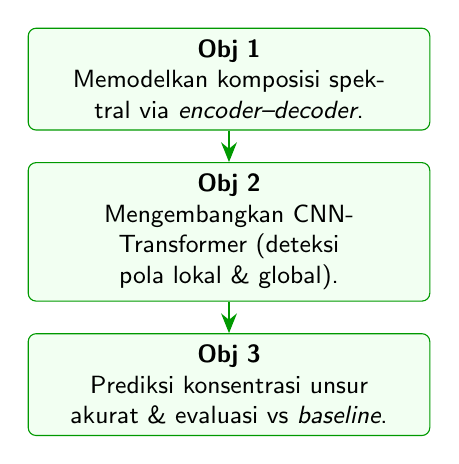
\begin{tikzpicture}[
        node distance=0.4cm,
        objbox/.style={rectangle, draw=green!60!black, fill=green!5, rounded corners=1mm,
          text width=4.8cm, align=center, font=\small\sffamily, minimum height=1.0cm, inner sep=1.5mm},
        arrow/.style={-{Stealth[length=2.5mm,width=2mm]}, thick, draw=green!60!black}
      ]
        \node[objbox] (obj1) {\textbf{Obj 1}\\Memodelkan komposisi spektral via \textit{encoder--decoder}.};
        \node[objbox, below=of obj1] (obj2) {\textbf{Obj 2}\\Mengembangkan CNN-Transformer (deteksi pola lokal \& global).};
        \node[objbox, below=of obj2] (obj3) {\textbf{Obj 3}\\Prediksi konsentrasi unsur akurat \& evaluasi vs \textit{baseline}.};
        
        \draw[arrow] (obj1) -- (obj2);
        \draw[arrow] (obj2) -- (obj3);
      \end{tikzpicture}
    \end{column}
  \end{columns}
\end{frame}

% =============================================================
% Slide 8: Proposed Framework Overview (3-Step Flow)
% =============================================================
\section{Methodology}

\begin{frame}{Proposed Framework Overview}
  \centering

  \tikzset{
    box/.style={rectangle, rounded corners, draw=black, fill=gray!10,
      text width=3.8cm, align=center, minimum height=1.5cm, font=\sffamily},
    arrow/.style={-{Stealth[length=3mm,width=2mm]}, thick}
  }
  \resizebox{0.95\linewidth}{!}{
  \begin{tikzpicture}[node distance=1.1cm and 1.5cm]
    \node[box] (phys) {\textbf{Data Sintetis}\\Saha--Boltzmann (LTE)\\Transisi NIST ASD};
    \node[box, right=of phys] (model) {\textbf{CNN--Transformer}\\Encoder--Decoder\\Cross-attention};
    \node[box, right=of model] (pred) {\textbf{Prediksi}\\Konsentrasi unsur\\Tanah vulkanik};
    \draw[arrow] (phys.east)--(model.west);
    \draw[arrow] (model.east)--(pred.west);
  \end{tikzpicture}
  }

  \vspace{0.3em}
  {\small
  \textbf{Why encoder--decoder?}
  \begin{itemize}\setlength{\itemsep}{2pt}
    \item Spektrum poliatom merupakan \emph{komposisi} dari spektrum monoatom.
    \item \textit{Cross-attention} memungkinkan decoder mempelajari aturan komposisi.
    \item CNN menangkap pola garis lokal; Transformer menangkap dependensi jarak jauh.
  \end{itemize}

  \vspace{0.2em}
  \textbf{Kerangka kerja (3 langkah):}
  \begin{enumerate}\setlength{\itemsep}{2pt}
    \item Membangkitkan spektrum sintetis mono \& poliatom (berbasis fisika).
    \item Melatih CNN--Transformer Encoder--Decoder dengan \textit{cross-attention}.
    \item Memvalidasi pada spektrum LIBS eksperimental tanah vulkanik.
  \end{enumerate}
  }
\end{frame}

% =============================================================
% Slide 9: Model Architecture (Pipeline Diagram)
% =============================================================
\begin{frame}{Model Architecture}
  \centering

  \tikzset{
    box/.style={rectangle, rounded corners, draw=black!40, fill=gray!10,
                text width=2.2cm, minimum height=0.65cm,
                align=center, font=\small\sffamily},
    cnn/.style={box, fill=uskGold!15, draw=uskGold!70},
    trans/.style={box, fill=airforceblue!15, draw=airforceblue,
                  minimum width=2.6cm},
    pred/.style={box, fill=maincolor!12, draw=maincolor,
                 minimum width=3.2cm, minimum height=0.8cm,
                 font=\small\sffamily\bfseries},
    arr/.style={-{Stealth[length=5pt]}, thick, black!60},
    lbl/.style={font=\scriptsize\itshape, text=airforceblue}
  }

  \begin{tikzpicture}[node distance=0.45cm and 0.6cm]
    % --- Jalur Encoder ---
    \node[box] (mono) {Spektrum\\Monoatom};
    \node[cnn, right=of mono] (cnn1) {1D CNN};
    \node[trans, right=of cnn1] (enc) {Transformer\\Encoder};

    % --- Jalur Decoder ---
    \node[box, below=1.3cm of mono] (poly) {Spektrum\\Poliatom};
    \node[cnn, right=of poly] (cnn2) {1D CNN};
    \node[trans, right=of cnn2] (dec) {Transformer\\Decoder};

    % --- Cross-attention ---
    \draw[arr, dashed] (enc.south) -- node[right, lbl]{cross-attention} (dec.north);

    % --- Prediksi ---
    \node[pred, right=0.9cm of $(enc.east)!0.5!(dec.east)$] (pred) {Prediksi\\Konsentrasi};

    \draw[arr] (mono) -- (cnn1);
    \draw[arr] (cnn1) -- (enc);
    \draw[arr] (poly) -- (cnn2);
    \draw[arr] (cnn2) -- (dec);
    \draw[arr] (enc.east) -- ++(0.25,0) |- (pred.west);
    \draw[arr] (dec.east) -- ++(0.25,0) |- (pred.west);
  \end{tikzpicture}

  \vspace{0.1em}

  {\small
  \begin{columns}[T,onlytextwidth]
    \begin{column}{0.31\textwidth}
      \textbf{CNN (Feature Extractor)}
      \begin{itemize}\setlength{\itemsep}{1pt}
        \item Konvolusi 1D pada panjang gelombang
        \item Menangkap profil puncak
        \item Ekstraksi pola lokal
      \end{itemize}
    \end{column}
    \begin{column}{0.31\textwidth}
      \textbf{Transformer Encoder}
      \begin{itemize}\setlength{\itemsep}{1pt}
        \item Input spektrum monoatom
        \item Self-attention
        \item Dependensi global
      \end{itemize}
    \end{column}
    \begin{column}{0.34\textwidth}
      \textbf{Transformer Decoder}
      \begin{itemize}\setlength{\itemsep}{1pt}
        \item Input spektrum poliatom
        \item Cross-attention dengan encoder
        \item Mempelajari aturan komposisi
      \end{itemize}
    \end{column}
  \end{columns}
  }
\end{frame}

% =============================================================
% Slide 10: Cross-Attention Mechanism (Key Idea)
% =============================================================
\begin{frame}{Mekanisme Kunci: Cross-Attention}
  \begin{block}{Ide Utama}
    {\small Cross-attention memungkinkan decoder mempelajari \emph{bagaimana spektrum poliatom tersusun dari komponen spektral monoatom}.}
  \end{block}

  \begin{columns}[T,onlytextwidth]
    \begin{column}{0.55\textwidth}
      {\small
      \textbf{Cara kerja (Masalah $\rightarrow$ Solusi):}
      \begin{itemize}\setlength{\itemsep}{2pt}
        \item \textbf{Ekstraksi fitur} $\rightarrow$ \textit{1D CNN} menangkap bentuk garis lokal.
        \item \textbf{Konteks monoatom} $\rightarrow$ \textit{Self-attention} membangun representasi per-unsur.
        \item \textbf{Pemodelan komposisi} $\rightarrow$ \textit{Cross-attention} meng-\textit{query} encoder untuk mengurai campuran poliatom.
        \item \textbf{Output} $\rightarrow$ Vektor konsentrasi unsur.
      \end{itemize}
      }
    \end{column}
    \begin{column}{0.42\textwidth}
      \centering
      \tikzset{
        block/.style={rectangle, rounded corners, draw=black!40, fill=gray!10,
          text width=3.0cm, align=center, minimum height=0.7cm, font=\scriptsize\sffamily}
      }
      \begin{tikzpicture}[node distance=0.35cm]
        \node[block] (q) {\textbf{Query}\\Fitur poliatom};
        \node[block, below=of q] (k) {\textbf{Key, Value}\\Fitur monoatom};
        \node[block, below=of k, fill=uskGold!12, draw=uskGold!60] (out) {\textbf{Output}\\Representasi komposisi};

        \draw[-{Stealth[length=4pt]}, thick, black!50] (q.south) -- (k.north);
        \draw[-{Stealth[length=4pt]}, thick, draw=maincolor] (k.south) -- (out.north);
      \end{tikzpicture}

      \vspace{0.2em}
      {\scriptsize Decoder meng-\textit{query} encoder untuk menemukan komponen monoatom mana yang menjelaskan spektrum poliatom.}
    \end{column}
  \end{columns}
\end{frame}

% =============================================================
% Slide 11: Sumber Data
% =============================================================
\section{Dataset \& Evaluation}

\begin{frame}{Sumber Data}
  \centering

  \tikzset{
    box/.style={rectangle, rounded corners, draw=black!40, fill=gray!10,
                minimum width=2.6cm, minimum height=0.65cm,
                align=center, font=\small\sffamily},
    arr/.style={-{Stealth[length=5pt]}, thick, black!60}
  }
  \begin{tikzpicture}[node distance=0.4cm and 0.7cm]
    \node[box] (sim) {Simulasi\\Fisika};
    \node[box, right=of sim] (syn) {Spektrum\\Sintetis};
    \node[box, right=of syn] (pre) {Pre-training};
    \node[box, right=of pre] (ft) {Fine-tuning};
    \node[box, below=0.4cm of ft] (exp) {LIBS\\Eksperimental};

    \draw[arr] (sim) -- (syn);
    \draw[arr] (syn) -- (pre);
    \draw[arr] (pre) -- (ft);
    \draw[arr] (exp) -- (ft);
  \end{tikzpicture}

  \vspace{0.4em}

  \begin{columns}[T,onlytextwidth]
    \begin{column}{0.48\textwidth}
      {\small
      \textbf{Spektrum Sintetis}
      \begin{itemize}\setlength{\itemsep}{2pt}
        \item Populasi Saha--Boltzmann pada kondisi LTE.
        \item Transisi atomik dari NIST ASD.
        \item $T$: 5000--15000\,K; $n_e$: $10^{16}$--$10^{18}$\,cm$^{-3}$.
        \item Spektrum mono \& poliatom terpisah.
        \item Digunakan untuk \textit{pre-training}.
      \end{itemize}
      }
    \end{column}
    \begin{column}{0.48\textwidth}
      {\small
      \textbf{Spektrum Eksperimental}
      \begin{itemize}\setlength{\itemsep}{2pt}
        \item LIBS pada sampel tanah vulkanik (wilayah Aceh).
        \item Kondisi laboratorium terkontrol.
        \item Referensi: XRF / ICP-OES sebagai \textit{ground truth}.
        \item Digunakan untuk \textit{fine-tuning} \& evaluasi akhir.
      \end{itemize}
      }
    \end{column}
  \end{columns}
\end{frame}

% =============================================================
% Slide 12: Evaluation Plan
% =============================================================
\begin{frame}{Evaluation Plan}
  \begin{columns}[T,onlytextwidth]
    \begin{column}{0.48\textwidth}
      {\small
      \textbf{Metrik Performa}
      \begin{itemize}\setlength{\itemsep}{3pt}
        \item \textbf{RMSE} --- besaran \textit{error} prediksi
          \[ \text{RMSE} = \sqrt{\frac{1}{n}\sum_{i=1}^{n}(y_i - \hat{y}_i)^2} \]
        \item \textbf{R\textsuperscript{2}} --- koefisien determinasi
          \[ R^2 = 1 - \frac{\sum(y_i - \hat{y}_i)^2}{\sum(y_i - \bar{y})^2} \]
        \item \textbf{MAPE} --- \textit{error} relatif
          \[ \text{MAPE} = \frac{1}{n}\sum\left|\frac{y_i - \hat{y}_i}{y_i}\right| \times 100\% \]
      \end{itemize}
      }
    \end{column}
    \begin{column}{0.48\textwidth}
      {\small
      \textbf{Perbandingan Baseline}
      \begin{itemize}\setlength{\itemsep}{3pt}
        \item CNN saja (tanpa Transformer)
        \item Transformer saja (tanpa CNN)
        \item Regresi konvensional (PLS, SVR)
        \item Informer (Walidain et~al., 2026)
      \end{itemize}

      \vspace{0.4em}
      \textbf{Strategi Validasi}
      \begin{itemize}\setlength{\itemsep}{3pt}
        \item $k$-fold cross-validation
        \item Transfer domain sintetis $\rightarrow$ eksperimental
        \item Akurasi konsentrasi per-unsur
      \end{itemize}
      }
    \end{column}
  \end{columns}
\end{frame}

% =============================================================
% Slide 13: Kontribusi Penelitian
% =============================================================
\begin{frame}{Research Contributions}
  \begin{block}{Scientific Contributions}
    \begin{enumerate}\setlength{\itemsep}{8pt}
      \item \textbf{Pemodelan spektral mono--poliatom}\\
      {\small Pendekatan pertama yang secara eksplisit memodelkan hubungan komposisi antara spektrum monoatom dan poliatom LIBS melalui mekanisme \textit{cross-attention}.}

      \item \textbf{Kerangka CNN--Transformer untuk analisis LIBS}\\
      {\small Arsitektur hibrida yang menggabungkan ekstraksi fitur lokal (CNN) dan pemodelan dependensi global (Transformer) dalam paradigma encoder--decoder.}

      \item \textbf{Karakterisasi tanah vulkanik}\\
      {\small Prediksi kuantitatif konsentrasi unsur pada matriks geologi kompleks, relevan untuk vulkanologi dan penilaian tanah pertanian.}
    \end{enumerate}
  \end{block}
\end{frame}

% =============================================================
% Slide 14: Research Timeline
% =============================================================
\begin{frame}{Research Timeline}
  \centering
  \tikzset{
    phase/.style={rectangle, rounded corners, draw=black!40, fill=gray!10,
                  minimum width=4.2cm, minimum height=0.8cm,
                  align=center, font=\small\sffamily},
    time/.style={font=\scriptsize, text=uskGold!80!black},
    arr/.style={-{Stealth[length=5pt]}, thick, black!50}
  }

  \begin{tikzpicture}[node distance=0.8cm and 1.2cm]
    \node[phase, fill=uskGold!8]  (p1) {\textbf{Persiapan Data}\\{\scriptsize Simulasi \& pengukuran LIBS}};
    \node[phase, right=of p1, fill=uskGold!12] (p2) {\textbf{Pengembangan Model}\\{\scriptsize Desain CNN--Transformer}};
    \node[phase, below=of p1, fill=uskGold!16] (p3) {\textbf{Pelatihan \& Optimasi}\\{\scriptsize Training, tuning hyperparameter}};
    \node[phase, right=of p3, fill=uskGold!20] (p4) {\textbf{Evaluasi \& Penulisan}\\{\scriptsize Analisis hasil, penulisan tesis}};

    \draw[arr] (p1) -- (p2);
    \draw[arr] (p2.south) -- ++(0,-0.15) -| (p3.north);
    \draw[arr] (p3) -- (p4);

    \node[time, above=2pt of p1] {Bulan 1--3};
    \node[time, above=2pt of p2] {Bulan 3--5};
    \node[time, below=2pt of p3] {Bulan 5--8};
    \node[time, below=2pt of p4] {Bulan 8--10};
  \end{tikzpicture}

  \vspace{0.3em}
  \small
  \renewcommand{\arraystretch}{1.15}
  \begin{tabular}{cl}
    \toprule
    \textbf{Fase} & \textbf{Kegiatan Utama} \\
    \midrule
    1 & Pembangkitan spektrum sintetis, pengumpulan sampel LIBS \\
    2 & Desain arsitektur, implementasi CNN--Transformer \\
    3 & Pelatihan model, optimasi hyperparameter \\
    4 & Evaluasi performa, perbandingan, penulisan tesis \\
    \bottomrule
  \end{tabular}
\end{frame}

% =============================================================
% Slide 15: Kesimpulan & Penutup
% =============================================================
\begin{frame}{Conclusions \& Strong Close}
  \begin{itemize}\setlength{\itemsep}{3pt}
    \item \textbf{Paradigma:} Kerangka encoder--decoder yang secara eksplisit memodelkan komposisi spektral mono--poliatom.
    \item \textbf{Arsitektur:} CNN untuk pola lokal + Transformer untuk dependensi global + \textit{cross-attention} untuk komposisi.
    \item \textbf{Aplikasi:} Analisis kuantitatif unsur tanah vulkanik melalui LIBS.
    \item \textbf{Prospek:} Domain adaptation, efek non-LTE, \textit{deployment} analisis \textit{real-time}.
  \end{itemize}
  \vspace{0.8em}
  \centering
  \Large \textbf{CNN--Transformer Encoder--Decoder}\\
  \large \textbf{+ cross-attention mono--poliatom}\\[0.3em]
  \large $\Rightarrow$ \textbf{Analisis LIBS yang akurat dan \textit{physics-aware}}
\end{frame}

% =============================================================
% Q&A
% =============================================================
\begin{frame}[plain,noframenumbering]{}
  \centering
  \vspace{0.5em}
  {\Huge \textcolor{uskGold}{\textbf{Terima Kasih!}}}

  \vspace{0.6em}
  {\Large Pertanyaan \& Diskusi}

  \vspace{1.0em}
  {\large \textcolor{uskGold}{\textbf{Kontak:}}}\\[0.3em]
  {\small
    \textbf{Birrul Walidain:} \texttt{birrul@mhs.usk.ac.id}\\
    \textbf{Nasrullah Idris:} \texttt{nasrullah.idris@usk.ac.id}
  }

  \vfill
  {\footnotesize \textcolor{gray}{\textbf{Pembimbing}}}\\[0.2em]
  {\scriptsize \textcolor{gray}{Prof.\ Dr.\ Eng.\ Nasrullah, S.Si., M.T.\ (Fisika) \quad\&\quad Dr.\ Khairun Saddami, S.T.\ (Teknik Komputer)}}
\end{frame}

\end{document}
